% Created 2019-08-08 Thu 20:18
% Intended LaTeX compiler: pdflatex
\documentclass[presentation]{beamer}
\usepackage[utf8]{inputenc}
\usepackage[T1]{fontenc}
\usepackage{graphicx}
\usepackage{grffile}
\usepackage{longtable}
\usepackage{wrapfig}
\usepackage{rotating}
\usepackage[normalem]{ulem}
\usepackage{amsmath}
\usepackage{textcomp}
\usepackage{amssymb}
\usepackage{capt-of}
\usepackage{hyperref}
\usepackage[newfloat]{minted}
\usepackage{caption}
\usetheme{default}
\usepackage{tikz}
\usetikzlibrary{positioning}
\definecolor{MRGGreen}{rgb}{0, 0.350, 0.200}
\graphicspath{{./figures/}}
\usetheme{default}
\author{Charles Margossian, Yi Zhang}
\date{StanCon 2019, Cambridge UK \\ August 2019}
\title{Population and ODE-based models \\ using Stan and Torsten}
\AtBeginSection[]{\begin{frame}<beamer>\frametitle{Outline}\tableofcontents[currentsection,hideallsubsections,subsubsectionstyle=hide]\end{frame}}
\hypersetup{
 pdfauthor={Charles Margossian, Yi Zhang},
 pdftitle={Population and ODE-based models \\ using Stan and Torsten},
 pdfkeywords={},
 pdfsubject={},
 pdfcreator={Emacs 25.3.1 (Org mode 9.1.3)}, 
 pdflang={English}}
\begin{document}

\maketitle
\begin{frame}{Outline}
\setcounter{tocdepth}{1}
\tableofcontents
\end{frame}


\section{Course information}
\label{sec:orgaf9428b}
\begin{frame}[label={sec:org2d36595}]{}
\begin{block}{Instructors}
\begin{itemize}
\item Charles Margossian
\begin{itemize}
\item Columbia University, Department of Statistics
\end{itemize}
\item Yi Zhang
\begin{itemize}
\item Metrum Research Group
\end{itemize}
\end{itemize}
\end{block}
\begin{block}{TA}
\begin{itemize}
\item Steve Bronder
\begin{itemize}
\item Capital One
\end{itemize}
\end{itemize}
\end{block}
\end{frame}
\begin{frame}[label={sec:org040622e}]{Outline}
\begin{block}{Day 1}
\begin{itemize}
\item Introduction and modeling framework
\item Pharmacometrics models
\item Ordinary differential equation(ODE) based models
\item Numerical ODE integrators
\end{itemize}
\end{block}
\begin{block}{Day 2}
\begin{itemize}
\item Population models
\item Group/Population ODE integrators and MPI parallelisation
\item Group/Population solvers and MPI parallelisation
\end{itemize}
\end{block}
\end{frame}
\begin{frame}[label={sec:orga7c033a}]{Logistics}
METWORX\texttrademark{}, cloud-based modeling \& simulation platform by Metrum Research Group.
\begin{latex}
\begin{center}
  
\includegraphics[width=3cm]{metworx}
\end{center}

\begin{figure}
  \centering
  \begin{minipage}{0.3\textwidth}
    \centering
    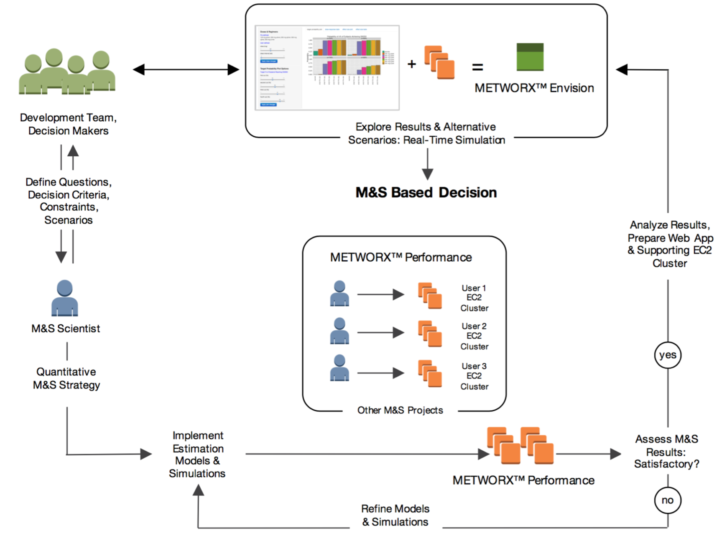
\includegraphics[width=0.9\textwidth]{metworx_efficiencies}
  \end{minipage}
  \begin{minipage}{0.3\textwidth}
    \centering
    
\includegraphics[width=0.9\textwidth]{metworx_desktop}
  \end{minipage}
  \begin{minipage}{0.3\textwidth}
    \centering
    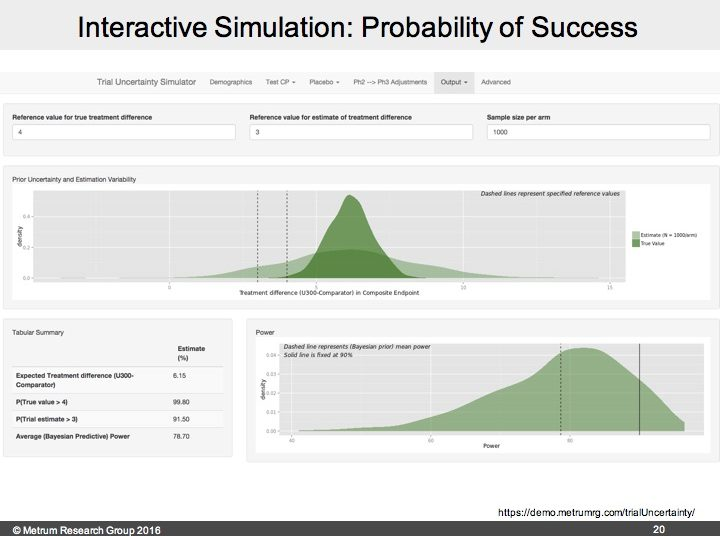
\includegraphics[width=0.9\textwidth]{metworx_decisionmakingtools}
  \end{minipage}
\end{figure}
\end{latex}
\end{frame}

\begin{frame}[label={sec:org01b4750}]{Logistics}
Workshop package
\begin{itemize}
\item R scripts and Stan files to do the exercises
\item These slides
\item Outline of the course
\item pAdditional documentation
\end{itemize}

We will be using:
\begin{itemize}
\item Torsten v0.87
\item RStan v2.19.2
\item ggplot, plyr, tidyr, dplyr
\end{itemize}
\end{frame}

\section{Introduction and modeling framework \\ \small{Charles Margossian}}
\label{sec:org94f5371}

\begin{frame}[label={sec:orge104f66}]{Preliminary question}
\begin{itemize}
\item Why Bayesian in a field such as pharmacometrics?
\item Example - \emph{Bayesian aggregation of average data: an application in drug development} \cite{Weber:2018}
\end{itemize}
\end{frame}

\begin{frame}[label={sec:orgef49733}]{Modeling framework}
\begin{block}{Box's loop}
\begin{latex}
\begin{figure}[htbp]
  \begin{center}
    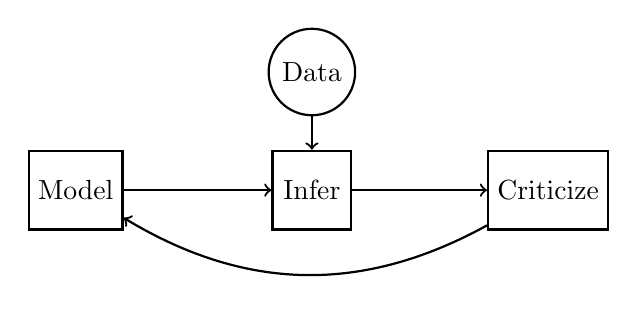
\begin{tikzpicture}
      [
      Box/.style={rectangle, draw=black!, fill=green!0, thick, minimum size=10mm},
      Gray/.style={rectangle, draw=black!, fill=gray!35, thick, minimum size=1mm},
      Round/.style={circle, draw=black!, fill=green!0, thick, minimum size=1mm},
      ]
      % Nodes
      \node[Round] (Data) at(0, 1.5) {Data};
      \node[Box] (Model) at(-3, 0) {Model};
      \node[Box] (Infer) at(0, 0) {Infer};
      \node[Box] (Crit) at (3, 0) {Criticize};

      % Lines
      \path [->, draw, thick] (Model) -- (Infer);
      \path [->, draw, thick] (Infer) -- (Crit);
      \path [->, draw, thick] (Crit) edge[bend left] (Model);
      \path [->, draw, thick] (Data) -- (Infer);

      % 

    \end{tikzpicture}
  \end{center}
\end{figure}
\end{latex}
\end{block}
\end{frame}

\begin{frame}[label={sec:orga13d3a1}]{Inference}
\begin{itemize}
\item find the set of parameters consistent with our model and our data
\item approximate this set with draws from the posterior distribution
\end{itemize}
\end{frame}
\begin{frame}[label={sec:org290978e}]{Sampling algorithm}
\begin{itemize}
\item Use the NUTS to sample \(\pi (\theta | y)\)
\item Requires users the specify \(\log \pi(\theta, y) = \log \pi(y | \theta) + \log \pi(\theta)\)
\end{itemize}
\end{frame}
\begin{frame}[label={sec:orgacee756}]{The "criticism" step}
This step can be broken up in two parts:
\begin{enumerate}
\item did we sample from the correct distribution?
\item does our model capture the characteristics of the data we care about?
\end{enumerate}
\end{frame}
\begin{frame}[label={sec:orgfa36135}]{Diagnosing the inference algorithm}
\begin{itemize}
\item look at the trace and the density plots
\item look at \(\hat R\) and effective number of samples
\item have any warning messages been issued, i.e. divergent transitions ?
\end{itemize}
\end{frame}
\begin{frame}[label={sec:org6d22fad}]{Example: fitting a linear model}
Likelihood:
\begin{align*}
  Y \sim \mathrm{Normal}(x \beta, \sigma^2)
\end{align*}

Prior:
\begin{align*}
  \beta \sim & \mathrm{Normal}(2, 1) \\
  \sigma^2 \sim & \mathrm{Normal}(1, 1)
\end{align*}
\end{frame}

\section{Numerical ODE integrators \\ \footnotesize{Yi Zhang}}
\label{sec:org7e6714e}

\begin{frame}[label={sec:org34848bd}]{Nonlinear ODEs without analytical solution}
\begin{block}{kinetics of an autocatalytic reaction \cite{robertson_numerical_1966}}
The structure of the reactions is 
\begin{equation*}
A \xrightarrow{k_1} B,\quad
B+B \xrightarrow{k_2} C + B,\quad
B+C \xrightarrow{k_3} C + A,
\end{equation*}
where \(k_1\), \(k_2\), \(k_3\) are the rate
constants and \(A\), \(B\) and \(C\) are the chemical species
involved. The corresponding ODEs are
\begin{align*}
x_1' &= -k_1x_1 + k_3x_2x_3\\
x_2' &=  k_1x_1 - k_2x_2^2 - k_3x_2x_3\\
x_3' &=  k_2x_2^2
\end{align*}
Given \(k_1=0.04, k_2=3.0e7, k_3=1.0e4\), we make inference
regarding the initial condition for \(x_1(t=0)\).
\end{block}
\begin{block}{Exercise}
Write Stan function for the above ODE's RHS.
\end{block}
\end{frame}

\begin{frame}[fragile,label={sec:org8cbacbf}]{Stan function for autocatalytic kinetics}
 \begin{align*}
x_1' &= -k_1x_1 + k_3x_2x_3\\
x_2' &=  k_1x_1 - k_2x_2^2 - k_3x_2x_3\\
x_3' &=  k_2x_2^2
\end{align*}

\begin{minted}[breaklines=true,fontsize=\footnotesize,breakanywhere=true]{stan}
functions{
  real[] reaction(real t, real[] x, real[] p, real[] r, int[] i){
    real dxdt[3];
    real k1 = p[1];
    real k2 = p[2];
    real k3 = p[3];
    dxdt[1] = -k1*x[1] + k3*x[2]*x[3];
    dxdt[2] =  k1*x[1] - k3*x[2]*x[3] - k2*(x[2])^2;
    dxdt[3] =  k2*(x[2])^2;
    return dxdt;
  }
}
\end{minted}
\begin{itemize}
\item What's the initial conditions for \(x_2\) and \(x_3\)?
\end{itemize}
\end{frame}

\begin{frame}[fragile,label={sec:org4b7195c}]{Numerical integrators}
 \begin{itemize}
\item Runge-Kutta 4th/5th (\texttt{rk45})
\begin{itemize}
\item non-stiff equations
\item Most popular, try this if you don't know the nature of the ODE, or what you're doing, or both.
\end{itemize}
\item Backward differentiation formula (\texttt{bdf})
\begin{itemize}
\item stiff equations
\item More expensive to use
\end{itemize}
\item Adams-Moulton
\begin{itemize}
\item non-stiff equations
\item higher-order of accuracy(do you really need it?)
\item scales better with number of steps
\end{itemize}
\end{itemize}
\end{frame}

\begin{frame}[fragile,label={sec:orgc6835fc}]{Numerical integrators}
 \begin{center}
\begin{tabular}{lll}
Integrators & Stan & Torsten\\
\hline
\texttt{rk45} & \texttt{integrate\_ode\_rk45} & \texttt{pmx\_integrate\_ode\_rk45}\\
\texttt{BDF} & \texttt{integrate\_ode\_bdf} & \texttt{pmx\_integrate\_ode\_bdf}\\
\texttt{Adams} & \texttt{integrate\_ode\_adams} & \texttt{pmx\_integrate\_ode\_adams}\\
\end{tabular}

\end{center}

\begin{minted}[breaklines=true,fontsize=\footnotesize,breakanywhere=true]{stan}
real[ , ] pmx_integrate_ode_rk45(ODE_RHS, real[] y0, real t0, real[] ts, real[] theta, real[] x_r, int[] x_i, real rtol = 1.e-6, real atol = 1.e-6, int max_step = 1e6);
\end{minted}
\begin{itemize}
\item \texttt{ODE\_RHS}: ODE right-hand-side \(f\) in \(y' = f(y, t, \theta, x_r, x_i)\).
\item \texttt{y0}: initial condition at time \texttt{t0}.
\item \texttt{t0}: initial time.
\item \texttt{ts}: times at which we require a solution.
\item \texttt{theta}: parameters to be passed to \(f\).
\item \texttt{x\_r}: real data to be passed to \(f\).
\item \texttt{x\_i}: integer data to be passed to \(f\).
\end{itemize}
\end{frame}


\begin{frame}[fragile,label={sec:orge3b7aa4}]{Exercise}
 \begin{itemize}
\item In each of 8 experiments performed \(x3\) is observed.
\item Hierarchical model for \(x0[1]\)
\end{itemize}
\begin{minted}[breaklines=true,fontsize=\footnotesize,breakanywhere=true]{stan}
model {
  x0_mu ~ lognormal(log(2.0), 0.5);    /* hyperparam */
  for (i in 1:nsub) {
    x0_1[i] ~ lognormal(x0_mu, 0.5);   /* loop each subject, sample initial condition */
  }
  sigma ~ cauchy(0, 1);                /* observation uncertainty */
  obs ~ lognormal(log(x3), sigma);
}
\end{minted}
\end{frame}

\begin{frame}[fragile,label={sec:orgb831eaa}]{Exercise}
 \begin{block}{Data available for the inference}
\begin{minted}[breaklines=true,fontsize=\footnotesize,breakanywhere=true]{stan}
data {
  int<lower=1> nsub;       /* nb. of subjects */
  int<lower=1> len[nsub];  /* nb. of results-extraction time points for each subject */
  int<lower=1> ntot;       /* total nb. of results-extraction time points */
  real ts[ntot];           /* concatenated array for results-extraction time points */
  real obs[ntot];          /* concatenated array for observed x3 */
}
\end{minted}
\end{block}

\begin{block}{Given above data and model, write the rest of Stan code.}
\begin{itemize}
\item Hint: see \texttt{chem.data.R} and \texttt{chem.init.R} .
\item Which numerical integrator are you using? Why?
\end{itemize}
\end{block}
\end{frame}

\begin{frame}[fragile,label={sec:org7679c9f}]{Exercise}
 How to build \& run?
\begin{block}{Edit/Add \texttt{cmdstan/make/local}}
\begin{minted}[breaklines=true,fontsize=\footnotesize,breakanywhere=true]{sh}
TORSTEN_MPI = 1  # flag on torsten's MPI solvers
CXXFLAGS += -isystem /usr/local/include    # path to MPI library's headers
\end{minted}
\end{block}
\begin{block}{Build in \texttt{cmdstan}}
\begin{minted}[breaklines=true,fontsize=\footnotesize,breakanywhere=true]{sh}
make ../example-models/examples/chemical_reactions/chem
\end{minted}
\end{block}
\begin{block}{Run}
\begin{minted}[breaklines=true,fontsize=\footnotesize,breakanywhere=true]{sh}
./chem sample adapt delta=0.95 random seed=1104508041 data file=chem.data.R init=chem.init.R
\end{minted}
\end{block}
\end{frame}

\section{ODE group integrators \\ \footnotesize{Yi Zhang}}
\label{sec:org60dfd0e}

\begin{frame}[fragile,label={sec:orgd16f8a2}]{ODE group integrators}
 \begin{center}
\begin{tabular}{ll}
Single ODE system & ODE group\\
\hline
\texttt{pmx\_integrate\_ode\_rk45} & \texttt{pmx\_integrate\_ode\_group\_rk45}\\
\texttt{pmx\_integrate\_ode\_bdf} & \texttt{pmx\_integrate\_ode\_group\_bdf}\\
\texttt{pmx\_integrate\_ode\_adams} & \texttt{pmx\_integrate\_ode\_group\_adams}\\
\end{tabular}

\end{center}

\begin{columns}
\begin{column}{0.45\columnwidth}
\begin{block}{Single ODE system}
\begin{minted}[breaklines=true,fontsize=\footnotesize,breakanywhere=true]{stan}
real[,]
pmx_integrate_ode_xxx(
      f,
      real[] y0, real t0,
      real[] ts,
      real[] theta,
      real[] x_r, int[] x_i,
      ...);
\end{minted}
\end{block}
\end{column}

\begin{column}{0.55\columnwidth}
\begin{block}{ODE group}
\begin{minted}[breaklines=true,fontsize=\footnotesize,breakanywhere=true]{stan}
matrix
pmx_integrate_ode_group_xxx(
     f,
     real[ , ] y0, real t0,
     int[] len, real[] ts,
     real[ , ] theta,
     real[ , ] x_r, int[ , ] x_i,
     ...);
\end{minted}
\end{block}
\end{column}
\end{columns}
\end{frame}

\begin{frame}[fragile,label={sec:orgcdd6cb7}]{ODE group integrators}
 \begin{columns}
\begin{column}{0.45\columnwidth}
\begin{block}{Single ODE system}
\begin{minted}[breaklines=true,fontsize=\footnotesize,breakanywhere=true]{stan}
real[ , ]
pmx_integrate_ode_xxx(
      f,
      real[] y0, real t0,
      real[] ts,
      real[] theta,
      real[] x_r, int[] x_i,
      ...);
\end{minted}
\end{block}
\end{column}

\begin{column}{0.55\columnwidth}
\begin{block}{ODE group}
\begin{minted}[breaklines=true,fontsize=\footnotesize,breakanywhere=true]{stan}
matrix
pmx_integrate_ode_group_xxx(
     f,
     real[ , ] y0, real t0,
     int[] len, real[] ts,
     real[ , ] theta,
     real[ , ] x_r, int[ , ] x_i,
     ...);
\end{minted}
\end{block}
\end{column}
\end{columns}
\begin{block}{}
\begin{itemize}
\item \texttt{len} specifies the length of data for each subject within
the above ragged arrays, and the size of \texttt{len} is the size
of the population.
\item The group integrators return a single matrix ragged
column-wise. The number of rows equals to the size of ODE system.
\end{itemize}
\end{block}
\end{frame}

\begin{frame}[fragile,label={sec:orgd399e3e}]{Exercise}
 \begin{block}{autocatalytic reaction model: ODE group version}
\begin{itemize}
\item Change the loop with the numerical integrator to use group
integrator.

\item Edit/Add \texttt{cmdstan/make/local}
\end{itemize}
\begin{minted}[breaklines=true,fontsize=\footnotesize,breakanywhere=true]{sh}
TORSTEN_MPI = 1  # flag on torsten's MPI solvers
CXXFLAGS += -isystem /usr/local/include    # path to MPI library's headers
\end{minted}
\begin{itemize}
\item Build in \texttt{cmdstan}
\end{itemize}
\begin{minted}[breaklines=true,fontsize=\footnotesize,breakanywhere=true]{sh}
make ../example-models/chemical_reactions/chem_group
\end{minted}
\begin{itemize}
\item Run
\end{itemize}
\begin{minted}[breaklines=true,fontsize=\footnotesize,breakanywhere=true]{sh}
mpiexec -n 2 -l ./chem_group sample adapt delta=0.95 random seed=1104508041 data file=chem.data.R init=chem.init.R
\end{minted}
\end{block}
\end{frame}

\begin{frame}[fragile,label={sec:org4b88d5e}]{Exercise}
 \begin{itemize}
\item What does output say?
\item How many cores can you use until performance saturates? Why?
\item Can you do it using Stan's \texttt{map\_rect}? Is there a
difference in style, output, and performance?
\end{itemize}
\end{frame}

\section{PMX population solvers \\ \footnotesize{Yi Zhang}}
\label{sec:org72b6b06}

\begin{frame}[fragile,label={sec:org6fe3e89}]{PMX population solvers}
 \begin{center}
\begin{tabular}{ll}
Single ODE system & ODE group\\
\hline
\texttt{pmx\_solve\_rk45} & \texttt{pmx\_solve\_group\_rk45}\\
\texttt{pmx\_solve\_bdf} & \texttt{pmx\_solve\_group\_bdf}\\
\texttt{pmx\_solve\_adams} & \texttt{pmx\_solve\_group\_adams}\\
\end{tabular}

\end{center}

\begin{columns}
\begin{column}{0.45\columnwidth}
\begin{block}{Individual solvers}
\begin{minted}[breaklines=true,fontsize=\footnotesize,breakanywhere=true]{stan}
matrix
pmx_solve_bdf(f, int nCmt,
  real[] time, real[] amt,
  real[] rate, real[] ii,
  int[] evid, int[] cmt,
  real[] addl, int[] ss,
  real[] theta, real[] biovar,
  real[] tlag, real rel_tol,
  real abs_tol, int max_step);
\end{minted}
\end{block}
\end{column}

\begin{column}{0.55\columnwidth}
\begin{block}{Population solvers}
\begin{minted}[breaklines=true,fontsize=\footnotesize,breakanywhere=true]{stan}
matrix
pmx_solve_group_bdf(f, int nCmt,
  int[] len, real[] time,
  real[] amt, real[] rate,
  real[] ii, int[] evid,
  int[] cmt, real[] addl,
  int[] ss, real[ , ] theta,
  real[ , ] biovar, real[ , ] tlag,
  real rel_tol, real abs_tol,
  int max_step);
\end{minted}
\end{block}
\end{column}
\end{columns}
\end{frame}


\begin{frame}[fragile,label={sec:orgd346cb4}]{PMX population solvers}
 \begin{minted}[breaklines=true,fontsize=\footnotesize,breakanywhere=true]{stan}
matrix
pmx_solve_group_bdf(f, int nCmt, int[] len, real[] time, real[] amt, real[] rate, real[] ii, int[] evid, int[] cmt, real[] addl, int[] ss, real[,] theta, real[,] biovar, real[,] tlag, real rel_tol, real abs_tol, int max_step);
\end{minted}

\begin{block}{}
\begin{figure}[htbp]
\centering
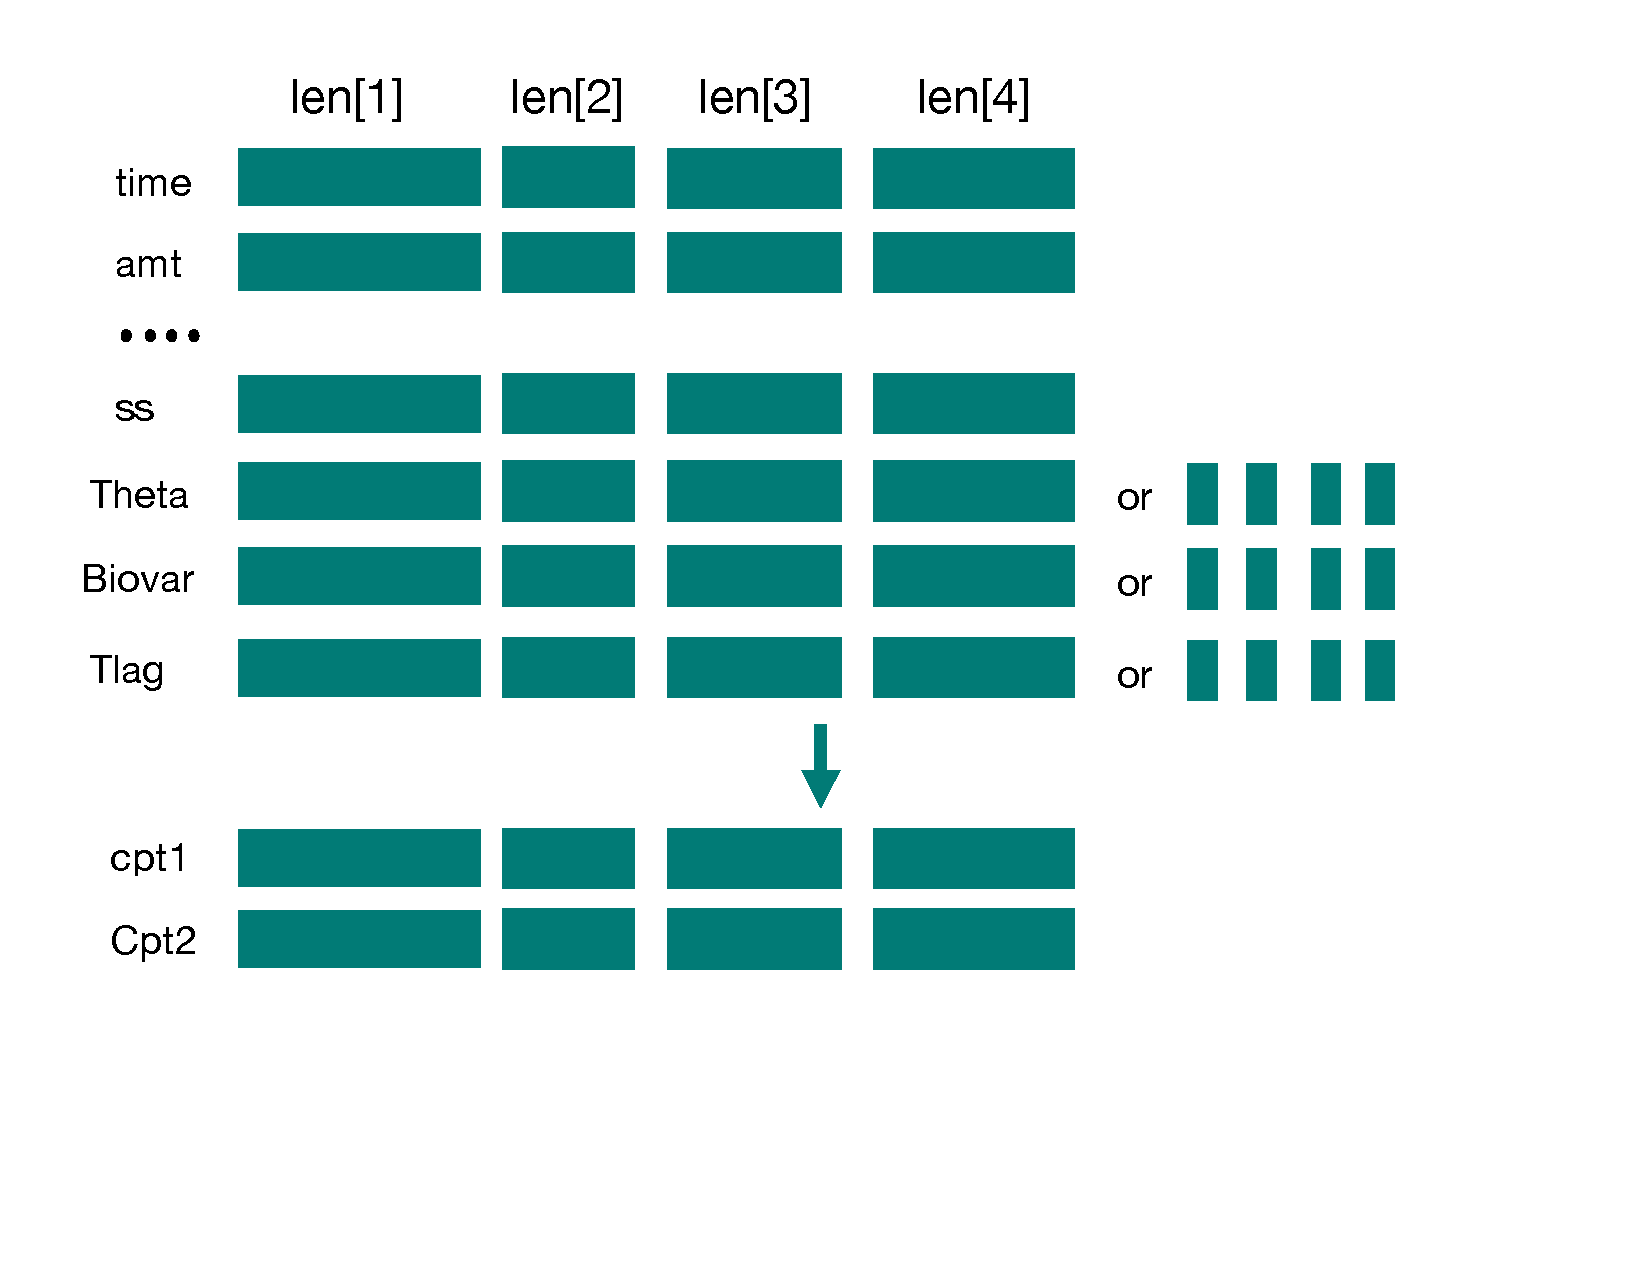
\includegraphics[width=0.6\textwidth]{./figures/group_solver_args.pdf}
\caption{arguments and output of \texttt{pmx\_solve\_group\_xxx}}
\end{figure}
\end{block}
\end{frame}

\begin{frame}[label={sec:orgf097975}]{Exercise}
We analyze the time to the first grade 2+ peripheral neuropathy
(PN) event in patients treated with an antibody-drug conjugate (ADC) delivering monomethyl auristatin E
(MMAE). We will simulate and analyze data using a simplified version of the
model reported in \cite{lu_time--event_2017}.
\begin{itemize}
\item Fauxlatuzumab vedotin 1.2 mg/kg IV boluses q3w \(\times\) 6 does.
\item 19 patients with 6 right-censored (simulated data).
\end{itemize}
\begin{columns}
\begin{column}{0.3\columnwidth}
\begin{block}{Model scheme}
\begin{center}
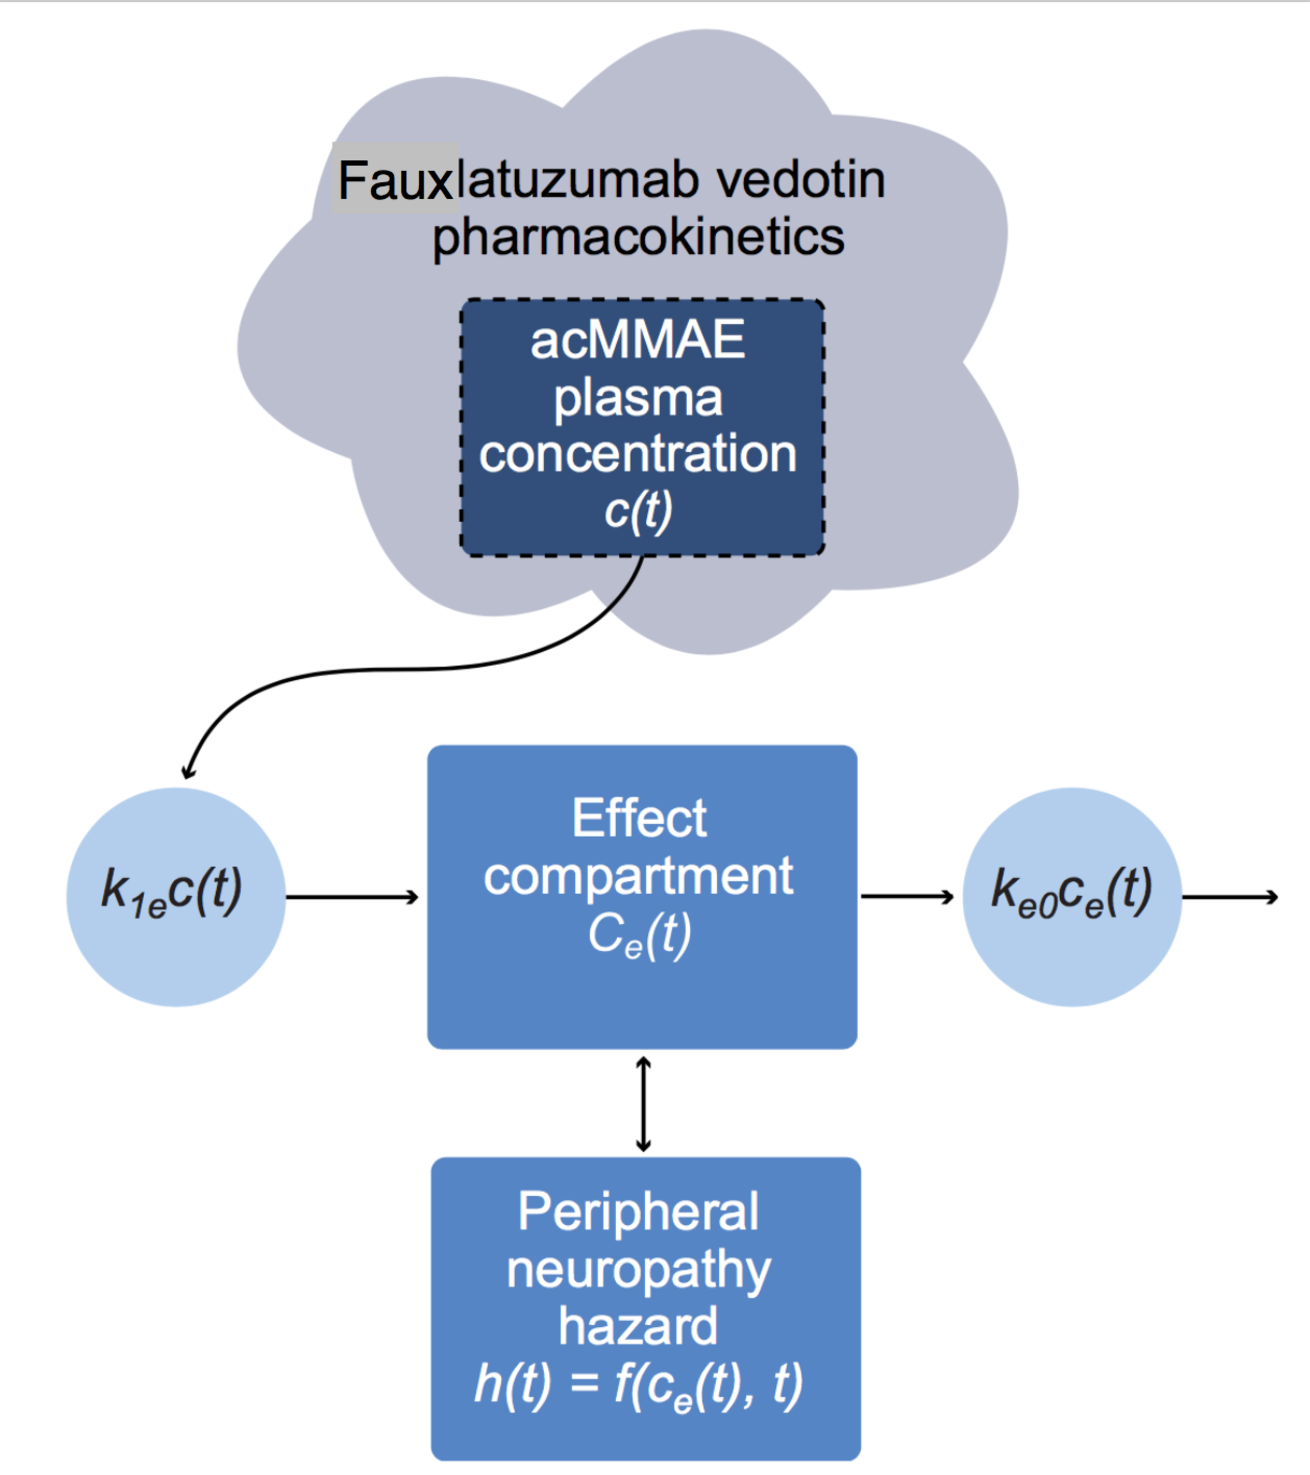
\includegraphics[width=0.9\columnwidth]{../../examples/ttpn2/lu2017Model.pdf}
\end{center}
\end{block}
\end{column}
\begin{column}{0.7\columnwidth}
\begin{block}{Note}
\begin{itemize}
\item To keep things simpler, we use the simulated individual CL and V values, and only model PD part of the problem.
\item PN hazard is substantially delayed relative to PK exposure.
\item Hazard increases over time to an extent not completely described by PK.
\end{itemize}
\end{block}
\end{column}
\end{columns}
\end{frame}

\begin{frame}[label={sec:org5156336}]{Exercise}
Likelihood for time to first PN \(\ge\) 2 event in the \(i^{th}\) patient:
\begin{align*}
\lefteqn{L\left(\theta | t_{\text{PN},i}, \text{censor}_i, X_i\right)} \\
  &= \left\{ \begin{array}{ll}
     h_i\left(t_{\text{PN},i} | \theta, X_i\right) e^{-\int_0^{t_{\text{PN},i}} h_i\left(u | \theta, X_i\right) du}, &
    \text{censor}_i = 0 \\
     e^{-\int_0^{t_{\text{PN},i}} h_i\left(u | \theta, X_i\right) du}, &
     \text{censor}_i = 1
\end{array} \right.
\end{align*}
where
 \begin{align*}
   t_{\text{PN}} &\equiv \text{time to first PN $\ge$ 2 or right
     censoring event} \\
 \theta &\equiv \text{model parameters} \\
 X &\equiv \text{independent variables / covariates} \\
 \text{censor} &\equiv \left\{ \begin{array}{ll}
     1, & \text{PN $\ge$ 2 event is right censored} \\
     0, & \text{PN $\ge$ 2 event is observed} 
 \end{array} \right.
\end{align*}
One can see the expression
\begin{equation*}
  e^{-\int_0^{t_{\text{PN},i}} h_i\left(u | \theta, X_i\right) du}
\end{equation*}
as the survival function at time \(t\).
\end{frame}

\begin{frame}[label={sec:orgd2c9df0}]{Exercise}
Hazard of PN grade 2+ based on the Weibull distribution,
with drug effect proportional to effect site concentration of MMAE:
\begin{align*}
  h_j(t) &= \beta E_{\text{drug}j}(t)^\beta t^{(\beta - 1)} \\
  E_{\text{drug}j}(t) &= \alpha c_{ej}(t) \\
  c^\prime_{ej}(t) &= k_{e0} \left(c_j(t) - c_{ej}(t)\right).
\end{align*}

Overall ODE system including integration of the hazard function:
\begin{align}
  x_1^\prime &= -\frac{CL}{V} x_1 \\
  x_2^\prime &= k_{e0} \left(\frac{x_1}{V} - x_2\right) \\
  x_3^\prime &= h(t)
  \end{align}
where \(x_2(t) = c_e(t)\) and \(x_3(t) = \int_0^t h(u) du\) aka cumulative hazard.
\end{frame}

\begin{frame}[fragile,label={sec:orgc4d135e}]{Exercise}
 \begin{block}{"just walk in a minute ago, literally" mode}
Apply \texttt{pmx\_solve\_group\_rk45} function
\end{block}
\begin{block}{Intermediate mode}
Code \texttt{pmx\_solve\_group\_rk45} function and its args. Use input data file \texttt{ttp2n.data2.R} as hint.
\end{block}
\begin{block}{hard mode}
Code ODE, \texttt{pmx\_solve\_group\_rk45} function and its args,
and the likelihood for harzard and censor event. Use input
data file \texttt{ttp2n.data2.R} and \texttt{model} block as hint.
\end{block}
\begin{block}{"why bother" mode}
\end{block}
\end{frame}

\begin{frame}[fragile,label={sec:orgb63939c}]{Exercise}
 \begin{block}{Edit/Add \texttt{cmdstan/make/local}}
\begin{minted}[breaklines=true,fontsize=\footnotesize,breakanywhere=true]{sh}
TORSTEN_MPI = 1         # flag on torsten's MPI solvers
CXXFLAGS += -isystem /usr/local/include # path to MPI library's headers
\end{minted}
\end{block}
\begin{block}{Build in \texttt{cmdstan}}
\begin{minted}[breaklines=true,fontsize=\footnotesize,breakanywhere=true]{sh}
make ../example-models/ttpn2/ttpn2_group
\end{minted}
\end{block}
\begin{block}{Run}
\begin{minted}[breaklines=true,fontsize=\footnotesize,breakanywhere=true]{sh}
mpiexec -n 4 -l ttpn2_group sample num_warmup=500 num_samples=500 data file=ttpn2.data2.R init=ttpn2.init.R
\end{minted}
\end{block}
\end{frame}

\begin{frame}[fragile,label={sec:org460dd0f}]{Exercise}
 \begin{itemize}
\item The parallel performance is not optimal, why?
\item Can you do it using Stan's \texttt{map\_rect}?
\end{itemize}
\end{frame}

\begin{frame}[label={sec:org9a5e265}]{Reference}
\bibliography{ttpn2}
\bibliographystyle{plain}
\end{frame}

\begin{frame}[label={sec:orge43443b}]{Reference}
\bibliography{./ref}
\bibliographystyle{apalike}
\end{frame}
\end{document}
